%%%%%%%%%%%%%%%%%%%%%%%%%%%%%%%%%%%%%%%%%%%%%%%%%%%%%%%%%%%%%%%%%
% Qualificacao de Doutorado / Dept Fisica, CFM, UFSC            %
% Eduardo@UFSC - 2015                                           %
%%%%%%%%%%%%%%%%%%%%%%%%%%%%%%%%%%%%%%%%%%%%%%%%%%%%%%%%%%%%%%%%%


%:::::::::::::::::::::::::::::::::::::::::::::::::::::::::::::::%
%                                                               %
%                          Capítulo 6                           %
%                                                               %
%:::::::::::::::::::::::::::::::::::::::::::::::::::::::::::::::%

%***************************************************************%
%                                                               %
%                      Conversão tauV - Gas                     %
%                                                               %
%***************************************************************%

\chapter{Estimando frações de gás}
\label{sec:gasfrac}

A fração de gás no modelo simples de evolução química ({\em closed-box model}) escala linearmente
com a metalicidade do gás, onde a inclinação da reta é o {\em yield}, que representa o quanto de
metais está sendo produzido e ejetado a cada geração de estrelas. Durante a pesquisa que nos levou a
escrever o artigo que está no Apênd. \label{apendice:GDetal2014b} encontramos uma relação
interessante que serviu de pontapé inicial para explorarmos a conversão de poeira em gás. Nesse
capítulo vamos comentar brevemente sobre nosso progresso e discutir quais os desafios enfrentados
até agora e aqueles que estão por vir nas próximas estapas de nosso projeto.

\section{Um modelo simples de evolução química}
\label{sec:gasfrac:closedbox}

A relação da qual comentamos no preambulo deste capítulo pode ser vista na Fig.
\ref{fig:dust2stars}. A razão entre o coeficiente de extinção e a densidade superficial de massa
estelar ($A_V / \mu_\star$) parece relacionar de maneira interessante com a metalicidade média das
populações estelares. 

\begin{figure}
	\centering
	%\resizebox{0.7\textwidth}{!}{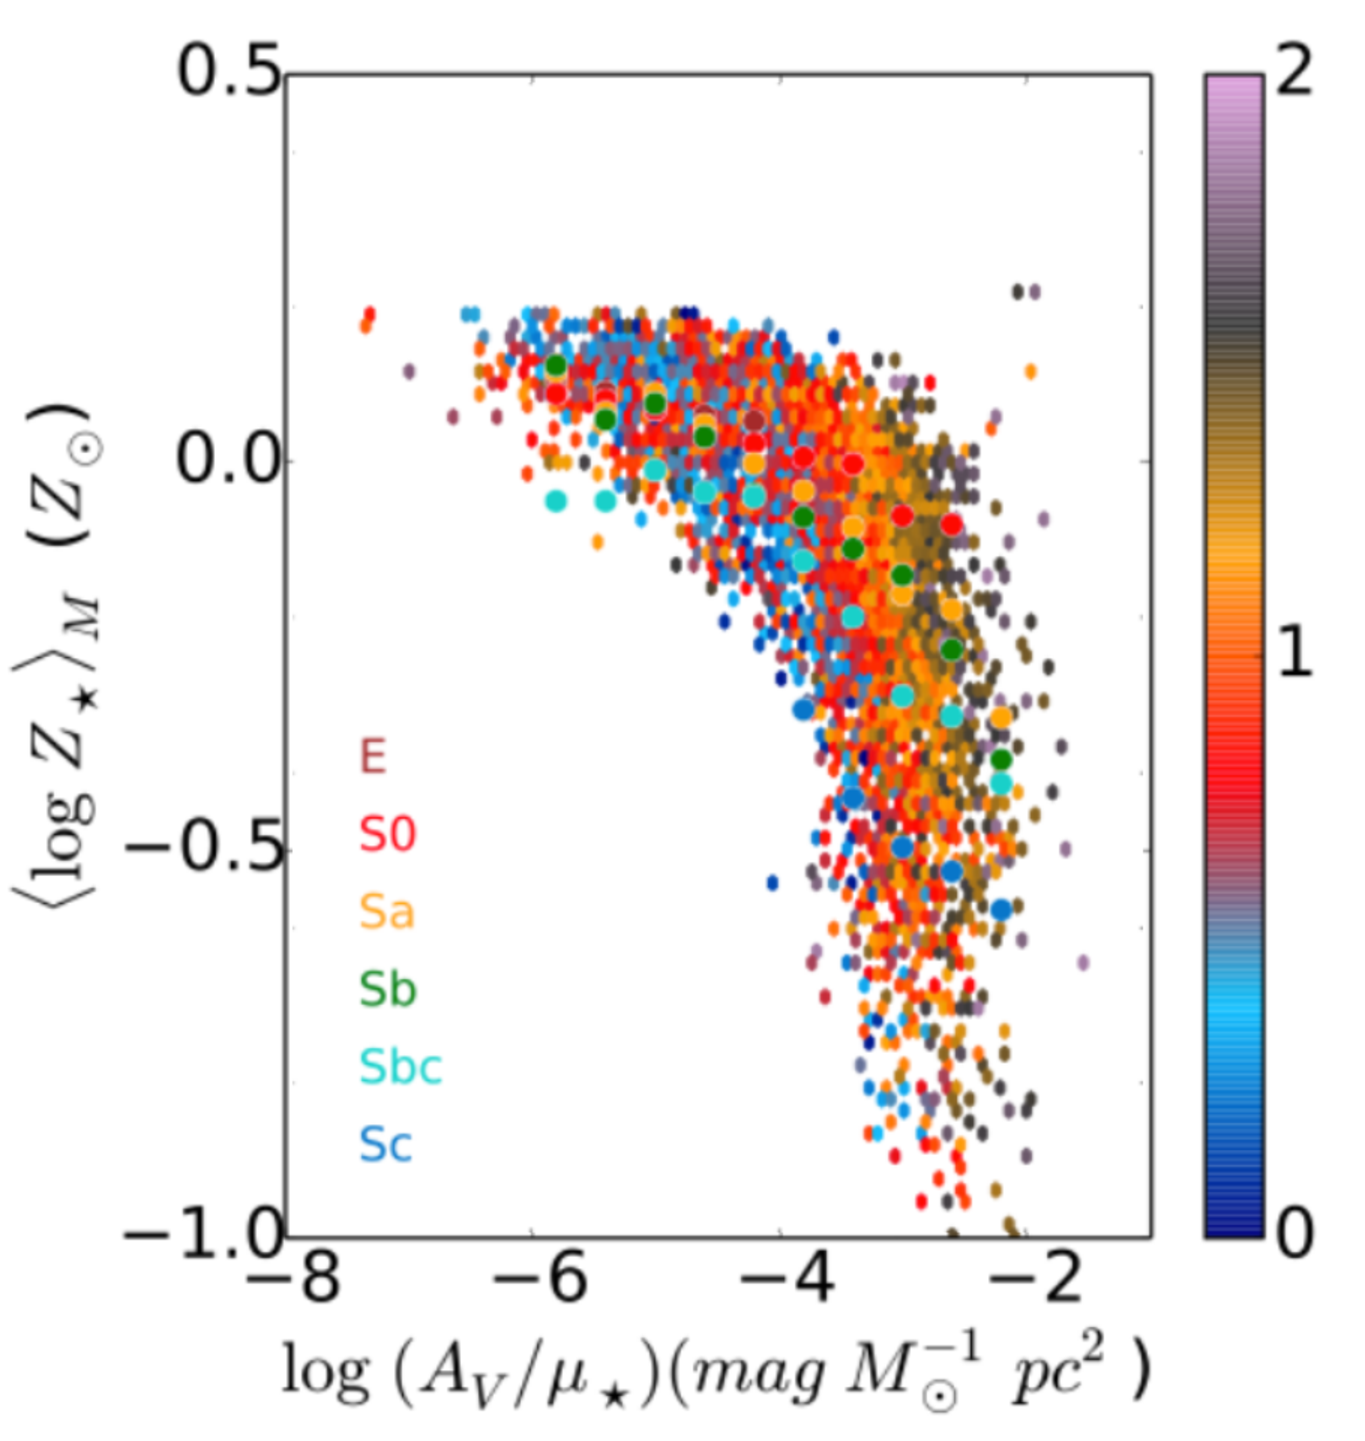
\includegraphics{figuras/dust2stars.pdf}}
	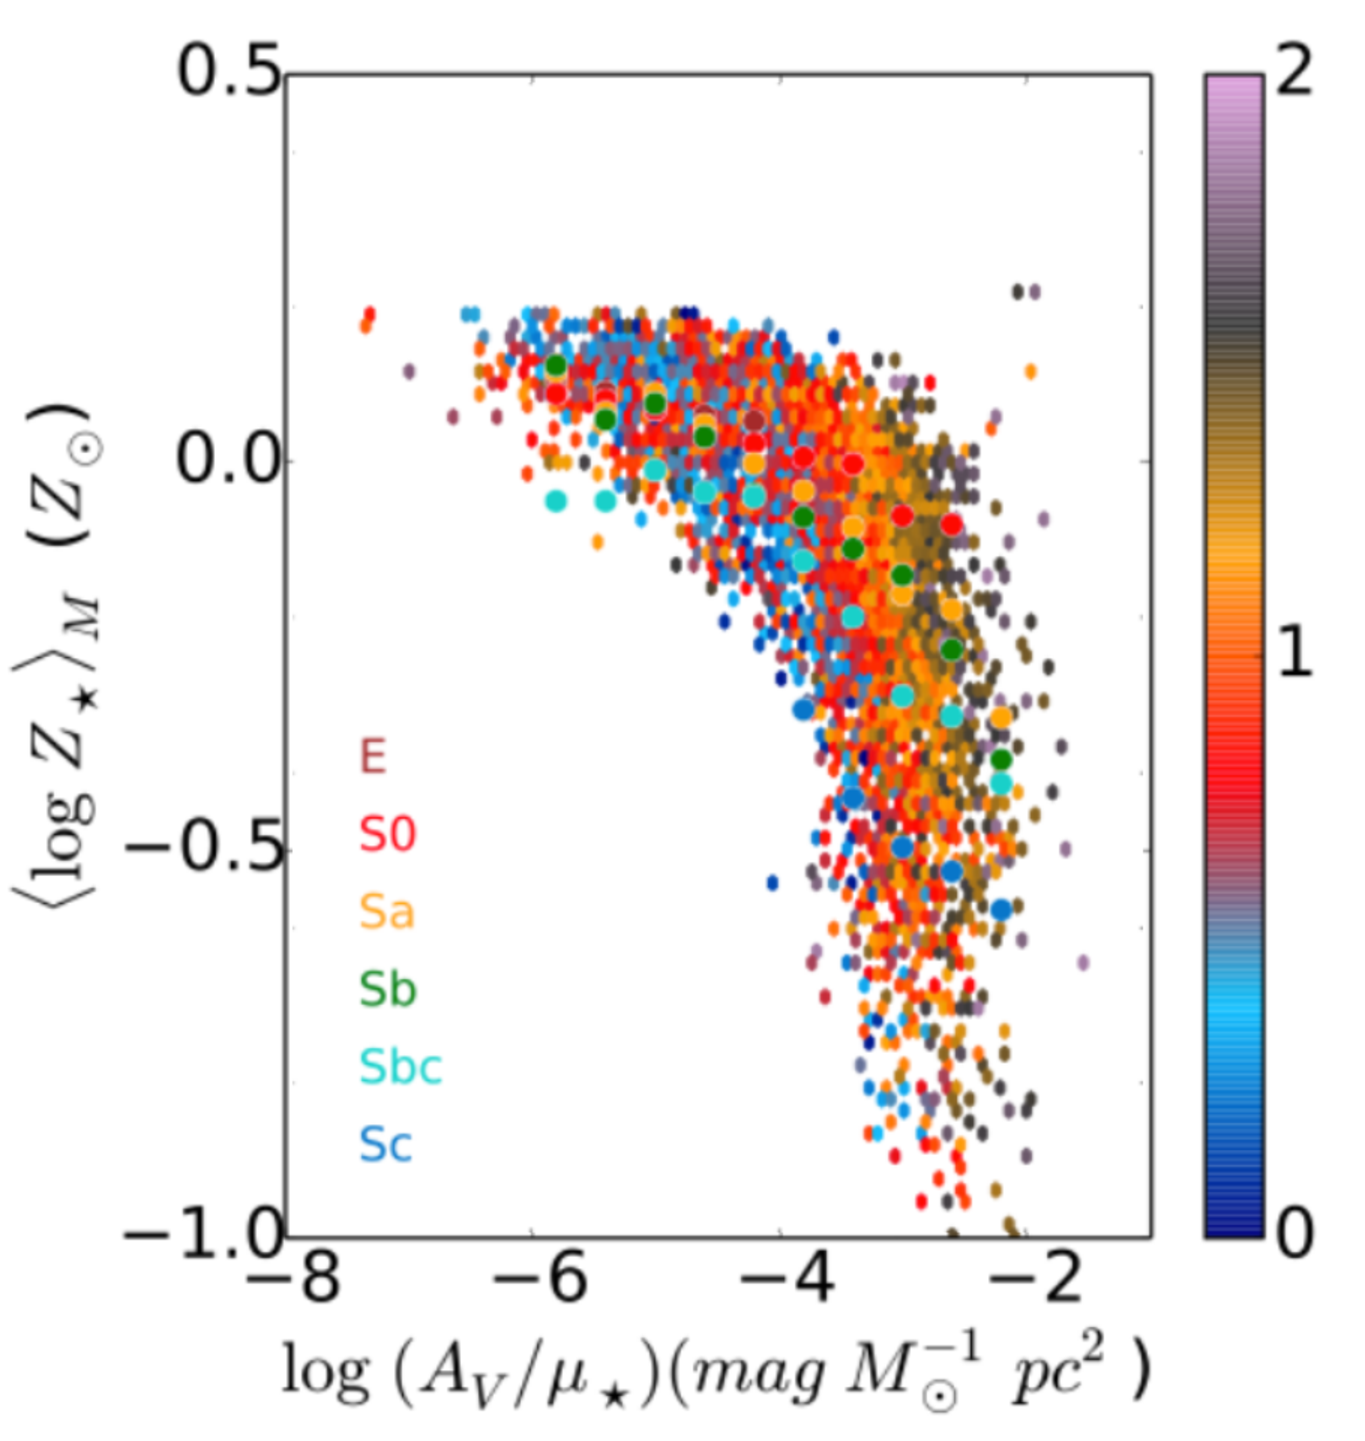
\includegraphics[height = 8cm, width = 9.5cm]{figuras/dust2stars.pdf}
	\caption[$A_V / \mu_\star$ vs. \meanM{\log Z_\stars}]
	{Relação entre metalicidade média das populações estelares e a razão entre o coeficiente de
extinção (em magnitude) e a densidade superficial de massa estelar. Os pontos são aproximadamente
6000 bins radiais de 300 galáxias (de 0 a 2 HLR divididos em 20 bins por galáxia) e estão
classificados em cores por tipo morfológico.}
	\label{fig:dust2stars}
\end{figure}

Podemos definir fração de gás como:
\begin{equation}
	f_{\mathrm{gas}}\ =\ \frac{M_{\mathrm{gas}}}{M_\star + M_{\mathrm{gas}}}\ =\ \frac{1}{1 +
	\left(\frac{M_\star}{M_{\mathrm{gas}}}\right)}\ \equiv\ \frac{1}{1 +
	\left(\frac{\mu_\star}{\SigmaGas}\right)}
	\label{eq:fgas}
\end{equation}
\noindent onde $M_{\mathrm{gas}}$ é a massa total na forma de gás e $M_\star$ é a massa total em
estrelas. 

Em um modelo simples de evolução química assume-se:
\begin{itemize}
	\setlength\itemsep{0.2cm}
  	\item onde não exista nem {\em inflow} nem {\em outflow} de gás na galáxia (isolada em um sistema
fechado sem entrada nem saída de gás);
  	\item seu gás inicial é totalmente pristino (sem presença de metais)
  	\item {\em Instant Recycling Approximation} - IRA: todas as estrelas com mais de 1 $M_\odot$
morrem imediatamente e todas as estrelas com massa menor que 1 $M_\odot$ vivem eternamente;
	\item a IMF é constante no tempo;
	\item o gas está sempre homogeneamente misturado.
\end{itemize}

Com estas simplificações, podemos escrever a metalicidade do gás como:
\begin{equation}
	Z_{\mathrm{gas}} = - y \ln f_{\mathrm{gas}},
	\label{eq:Zgas_closedbox}
\end{equation}
\noindent onde $y$ é o {\em yield} estelar (também conhecido como {\em true yield}). Nesta equação,
$Z$ e $y$ podem ser utilizados trocando Z pela abundância de um elemento específico e seu {\em
yield}. Invertendo a Eq. \ref{Zgas_closedbox} podemos definir o {\em yield} efetivo ($y_{eff}$), ou
seja, aquele que um sistema teria caso se comportasse como dito modelo ao longo de toda a linha do tempo. Essa
primeira equação foi derivada explicitamente pela primeira vez por \citet{Searle.Sargent.1972a} ao
estudar duas regiões \Hii gigantes, ditas ``isoladas''. \citet{Garnett.2002a}, assumindo que o {\em
true yield} seja constante, calcula $y_{eff}$ para 31 galáxias espirais e 13 galáxias irregulares,
encontrando valores distintos entre elas, o que o leva a concluir que o fluxo de gás ({\em outflow}
e {\em inflow}) nestes sistemas são ambos processos muito importantes para a evolução química de uma
galáxia. \citet{Tremonti.etal.2004a} calculam o $y_{eff}$ para $\sim 55000$ galáxias {\em
star-forming} do \SDSS, chegando a um valor de 0.0104. Ao adicionar outras medidas verifica que este
valor varia em uma escala de $\sim 10$ vezes, o que falha com a assunção de um {\em yield}
constante.

\section{Relação de Kennicut-Schmidt e nossa {\em pseudo-KS}}
\label{sec:gasfrac:KS}

Como explicado na Sec. \ref{sec:intro:galaxias}, a quantidade de gás de uma galáxia e a taxa de
formação estelar estão relacionadas através de uma lei de potências. Já a relação entre poeira e gás
é resultado direto da lei de Kennicut-Schmidt, que faz a ligação entre gás e formação estelar e da
relação entre gás e poeira \citep[][e suas referências]{Magdis.etal.2011a, Leroy.etal.2011a,
Santini.etal.2014a}. Pensando nisso, estabelecemos uma relação entre poeira e formação estelar, que
pode ser vista na Fig. \ref{fig:pseudoKS}. No painel esquerdo usamos $\tauVS$ como variável
representante da poeira e no direito, $\tauVN$. A conversão de poeira em gás é, da mesma forma que a
conversão de CO em gás, dependente da metalicidade, mas com a vantagem de não necessitarmos
medidas adicionais. O espalhamento nesta figura nos mostra que podemos explorar os resíduos em torno
desse ajuste.

\begin{figure}
	\centering
	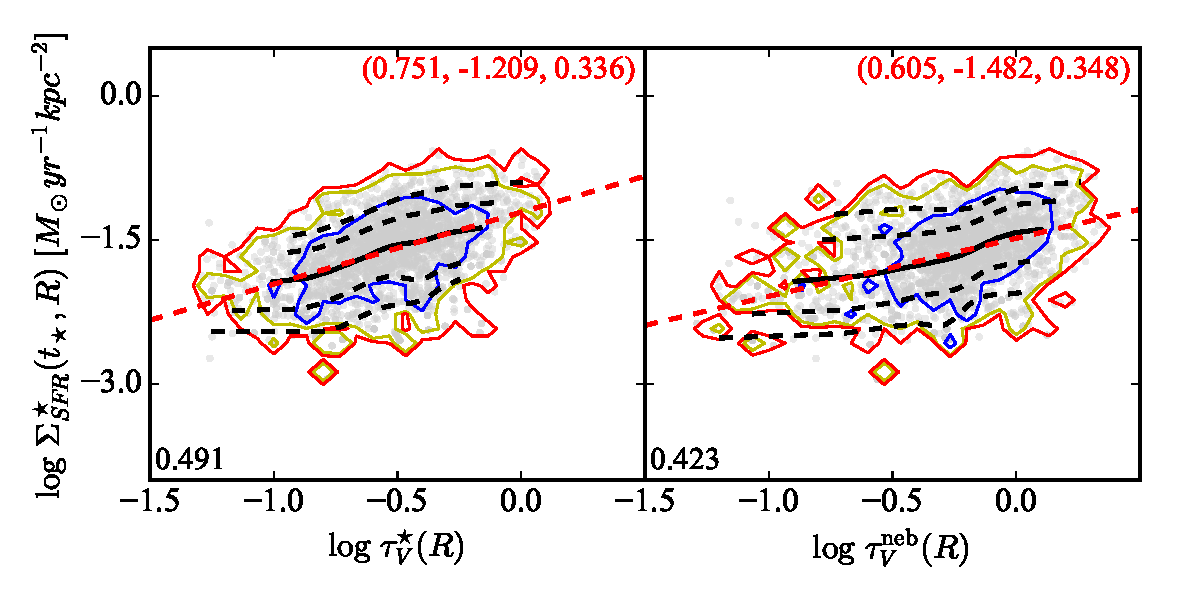
\includegraphics[width=0.95\textwidth]{figuras/pseudoKS.pdf}
	\caption[Nossa {\em pseudo-KS}.]
	{Relação entre a densidade superficial da taxa de formação estelar e o coeficiente de extinção
proveniente da síntese ($\tauVS$ - {\em painel esquerdo}) e do decremento de Balmer ($\tauVN$ -
{\em painel direito}). A linha tracejada em vermelho marca o ajuste linear da mediana e os
valores marcam o coeficiente de correlação de Spearmann (canto inferior esquerdo) e a
inclinação, valor de interceptação do eixo y e o valor do desvio médio quadrático da distribuição em
torno do ajuste (canto superior direito).}
	\label{fig:pseudoKS}
\end{figure}

\subsection{Resíduos da pseudo-KS}
\label{sec:gasfrac:KS:resid}
 
De todas as propriedades que vemos na Fig. \ref{fig:pseudoKSresid} é notável a participação da
metalicidade nebular no espalhamento na relação $\SigmaSFR$-$\tauVS$. Como segunda maior causadora
vem a fração em luz de populações jovens. O procedimento apresentado no Cap. \ref{sec:difextin}
talvez possa diminuir a influência de $x_Y$ (e também de $b/a$) em $\tauVS$ de maneira que tenhamos
um coeficiente de extinção mais diretamente ligado às regiões de formação estelar (portanto, mais
relacionado ao gás $H_2$). A correlação com o raio deve ter o mesmo fundamento que a com a densidade
superficial de massa estelar, visto que ambos estão fortemente ligados. A metalicidade estelar e a
idade média das populações estelares parecem assumirem um papel pequeno no espalhamento da pKS. Não
verificamos influência alguma da morfologia. Esses resultados se sustentam em parte quando
analisamos em uma escala menor, ou seja, zona a zona (Fig. \ref{fig:pseudoKSresidZonas}). A
influência de $x_Y$ nesta escala se torna majoritária aparecendo também uma correlação com a idade
média das populações estelares.

\begin{figure}
	\centering
	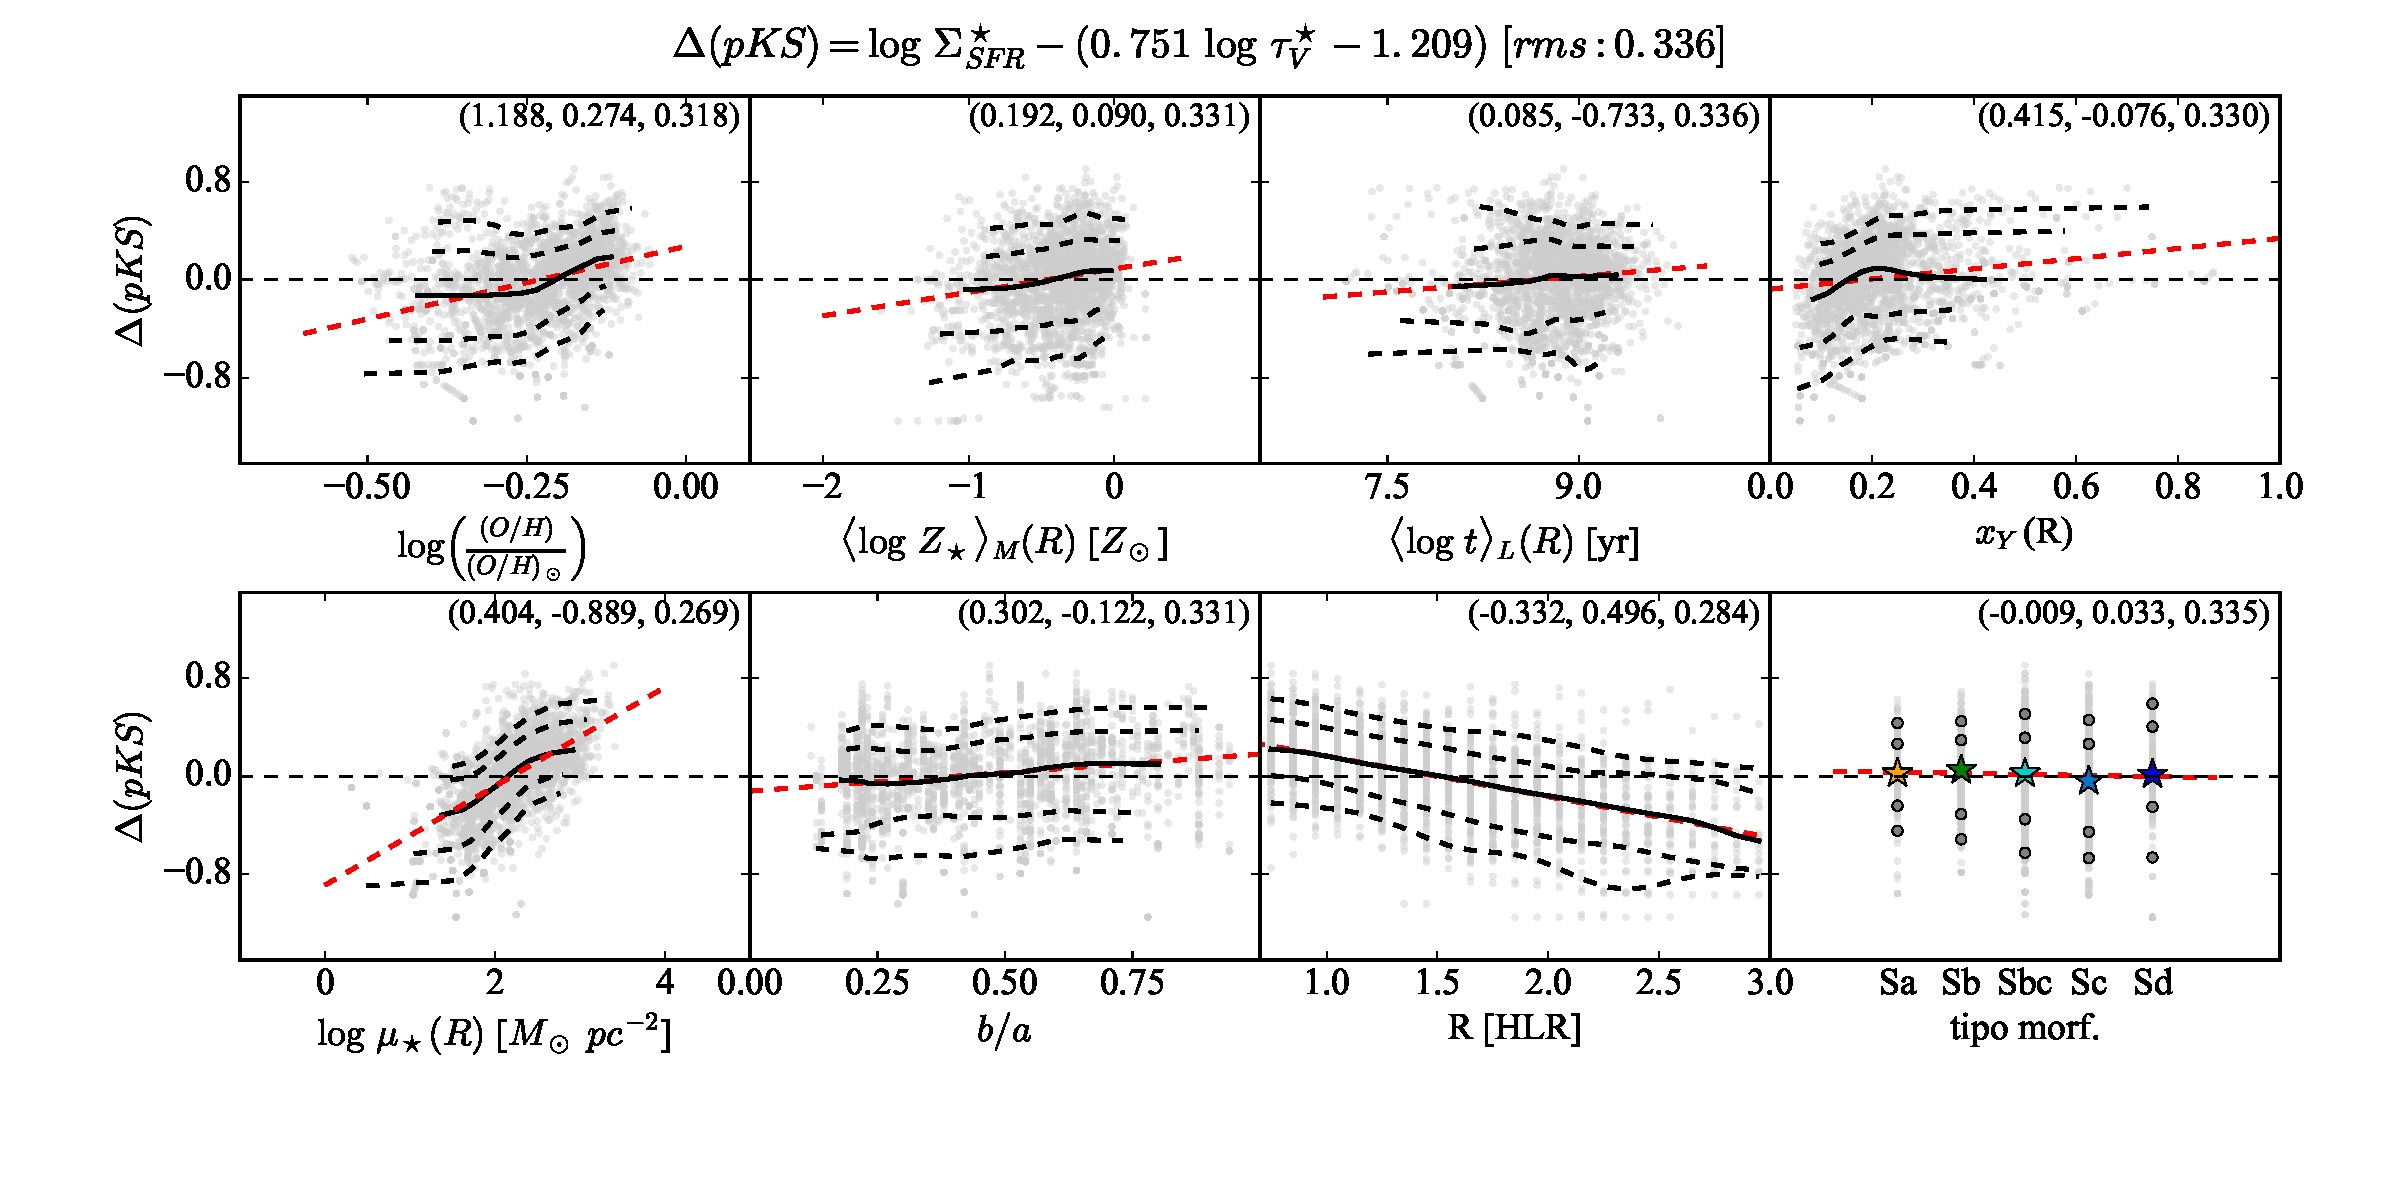
\includegraphics[width=0.99\textwidth]{figuras/deltapKS.pdf}
	\caption[Resíduos da {\em pseudo-KS}.]
	{No eixo y de todos os painés temos $\Delta_{pKS} = \SimgaSFR - (0.779 \tauVS - 1.191)$, onde, o
termo entre parenteses é o ajuste linear da mediana no painel esquerdo da Fig. \ref{fig:pseudoKS}.
No eixo x temos, na primeira fila, da esquerda para direita: metalicidade nebular ($12 + \log
(O/H)$), metalicidade estelar média pesada pela massa ($\meanM{\log Z_\star}$), idade média das
populações estelares ($\meanL{\log t_\star}$), fração em luz das populações estelares jovens
($x_Y$); na última fila, na mesma ordem: densidade superficial de massa estelar, relação axial, raio
e tipo morfológico.}
	\label{fig:pseudoKSresid}
\end{figure}

\begin{figure}
	\centering
	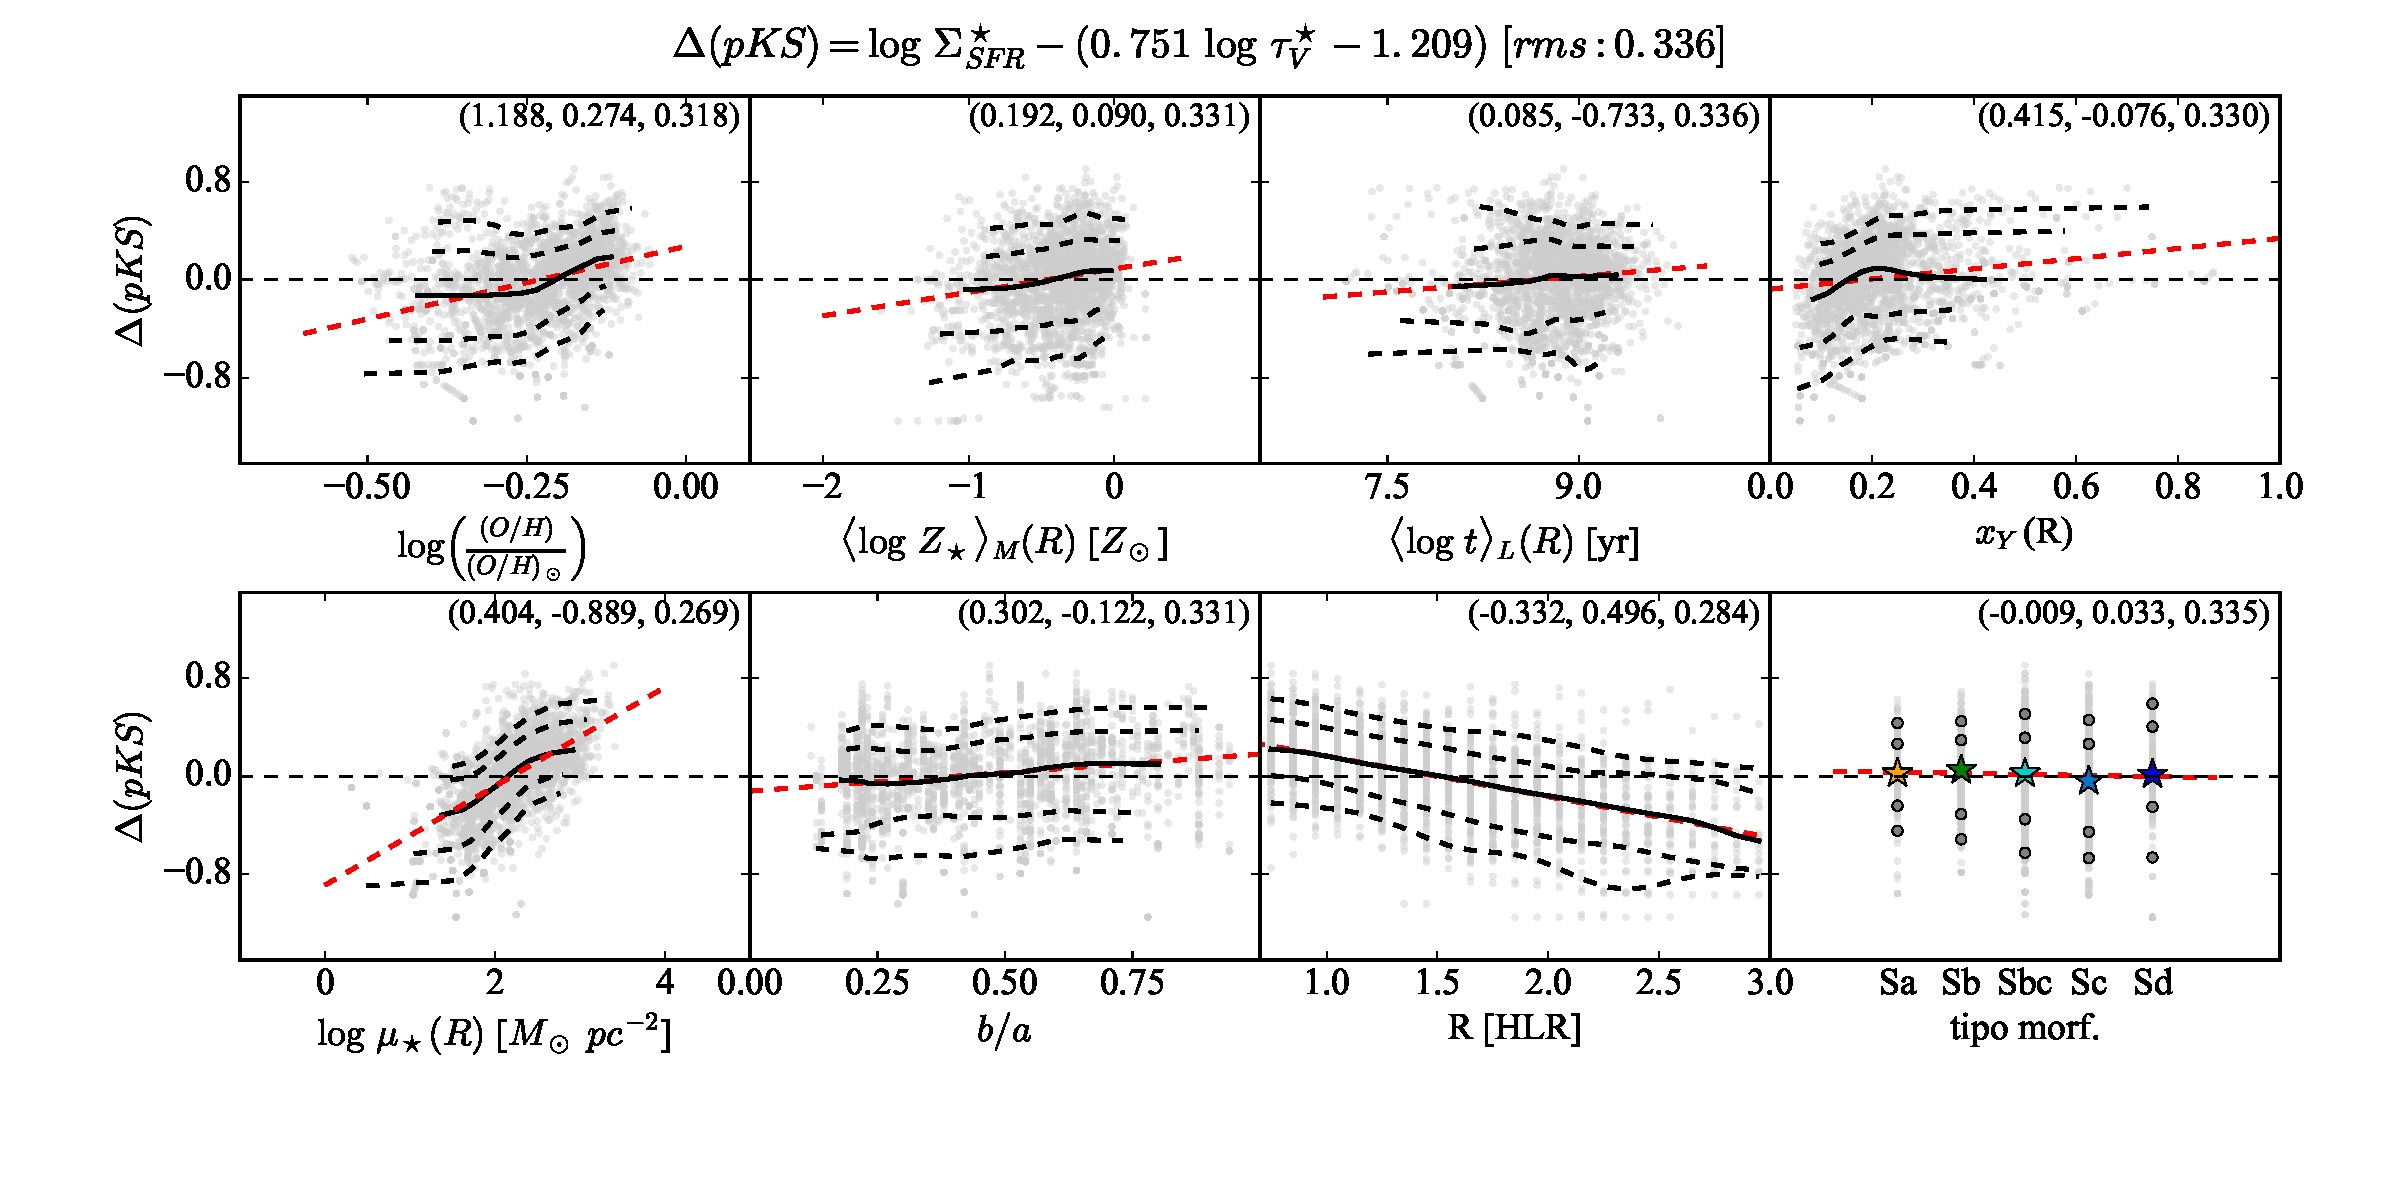
\includegraphics[width=0.99\textwidth]{figuras/deltapKS.pdf}
	\caption[Resíduos da {\em pseudo-KS}.]
	{Igual a Fig. \ref{fig:pseudoKSresid}, mas analisando zona a zona.}
	\label{fig:pseudoKSresidZonas}
\end{figure}

Diversos autores atualmente calculam e discutem a relação KS e a sua validade para diferentes
resoluções espaciais \citep[e.g., ][]{Kennicutt.etal.2007a, Leroy.etal.2012a,
Calzetti.Liu.Koda.2012a, Lada.etal.2013a, Tacconi.etal.2013a, Casasola.etal.2015a}. A inclinação
da KS (N = 1.4 na Eq. \ref{eq:SFRKennicutt}) varia geralmente entre 1 e 2, dependendo da resolução
espacial observada (regiões \Hii, perfis radiais, galáxias integradas) ou do tipo de gás usado
(atômico, molecular ou a soma dos dois).

\section{Conversão de poeira em gás.}
\label{sec:gasfrac:gas2dust}

Para converter poeira em gás primeiro precisamos da densidade superficial de poeira, que pode ser
conseguida utilizando a equação:
\begin{eqnarray}
	\tau_{\mathrm{d}} &=& \sigma_{\mathrm{d}} \int n_{\mathrm{d}} dz =
	\frac{\sigma_{\mathrm{d}}}{m_{\mathrm{d}}}\times\Sigma_{\mathrm{d}}
	\\
	\Sigma_{\mathrm{d}} &=& \frac{m_{\mathrm{d}}}{\sigma_{\mathrm{d}}}\ \tau_{\mathrm{d}},
	\label{eq:sigmadust}
\end{eqnarray}
\noindent onde $\sigma_{\mathrm{d}}$ é área de um grão de poeira, $n_{\mathrm{d}}$ é o número de
grãos de poeira ao longo de uma profundidade $dz$ e $m_{\mathrm{d}}$ é a massa de um grão de
poeira. Substituindo a Eq. \ref{eq:sigmadust} na Eq. \ref{eq:dust2gas} e assumindo $\tauV$ como
$\tau_{\mathrm{d}}$ obtemos:
\begin{equation}
	\SigmaGas\ =\ \kappa \times \frac{m_{\mathrm{d}}}{\sigma_{\mathrm{d}}}\ \tauV. 
	\label{eq:dust2gas_tauV}
\end{equation}

A conversão de poeira em gás é dependente da metalicidade segundo podemos verificar em todas as
referências sobre o assunto. Vamos explorar a conversão de poeira em gás em BR13, onde os autores
seguem o modelo de extinção de \citet{Charlot.Fall.2000a} e identificam algumas variáveis que vamos
utilizar:
\begin{eqnarray}
	\xi &=& \frac{\Sigma_{\mathrm{d}}}{\Sigma_Z} \\
	Z &=& \frac{\Sigma_Z}{\SigmaGas}  \\
	\delta_{\mathrm{DGR}} &=& \frac{\Sigma_{\mathrm{d}}}{\Sigma_Z}\ \frac{\Sigma_Z}{\SigmaGas}\ =\
\frac{\Sigma_{\mathrm{d}}}{\SigmaGas} = \xi Z,
	\label{eq:deltaDGR}
\end{eqnarray}
\noindent onde $\xi$ é a razão poeira-metais ({\em dust-to-metals}), Z é a metalicidade do gás e o
termo $\delta_{\mathrm{DGR}}$ é igual a $1/\kappa$. Utilizando a Eq. \ref{eq:deltaDGR} na Eq.
\ref{eq:dust2gas_tauV} e fazendo $m_{\mathrm{d}}/\sigma_{\mathrm{d}} \approx 0.2$, que corresponde
ao tipo de poeira Galáctica (BR13), temos:
\begin{equation}
	\SigmaGas\ \approx\ 0.2 \frac{\tauV}{\delta_{\mathrm{DGR}}}\ [M_\odot pc^{-2}].
	\label{eq:SigmaGasBR}
\end{equation}
Neste artigo os autores utilizaram dados de $\sim 70000$ galáxias {\em star-forming} do
\textit{SDSS}-DR7 e parametrizam $\delta_{\mathrm{DGR}}$ como a Eq. 28 de BR13:
\begin{equation}
	\delta_{\mathrm{DGR}}\ =\ (5.3 \times 10^{-3} - 1.1 \times 10^{-2})
\left(\frac{(O/H)}{(O/H)_\odot}\right),
	\label{eq:DGR_brinch_eq28}
\end{equation}
\noindent onde os fatores que multiplicam a metalicidade representam um intervalo onde esta
conversão é válida. O valor de $\delta_{\mathrm{DGR}}$ foi parametrizado utilizando as metalicidades
MPA/JHU\footnote{\href{http://wwwmpa.mpa-garching.mpg.de/SDSS/}{http://wwwmpa.mpa-garching.mpg.de/SDSS/}}
calculadas para o \SDSS. Para que possamos utilizar essa conversão, calibramos a abundância de
oxigênio de M13 com aquela utilizada no trabalho de BR13. Podemos ver na Fig. \ref{fig:calibZ} a
calibração feita utilizando 4 ajustes. Escolhemos utilizar o ajuste linear, pois é aquele com menor
desvio quadrático médio. Finalmente, nossa equação final para $\delta_{\mathrm{DGR}}$ é:
\begin{equation}
	\delta_{\mathrm{DGR}} =  (5.3 \times 10^{-3} - 1.1 \times 10^{-2}) \times 10^{\left(2.016 x\ +\ 0.425\right)},
	\label{eq:myDGR}
\end{equation}
\noindent onde $x = \log\ ((O/H)/(O/H)_\odot)$ de M13. Agora, substituindo a Eq. \ref{eq:myDGR} em
\ref{eq:SigmaGasBR} e utilizando este resultado na Eq. \ref{eq:fgas} podemos estimar frações de
gás para galáxias do \CAL. 
\begin{figure}
	\centering
	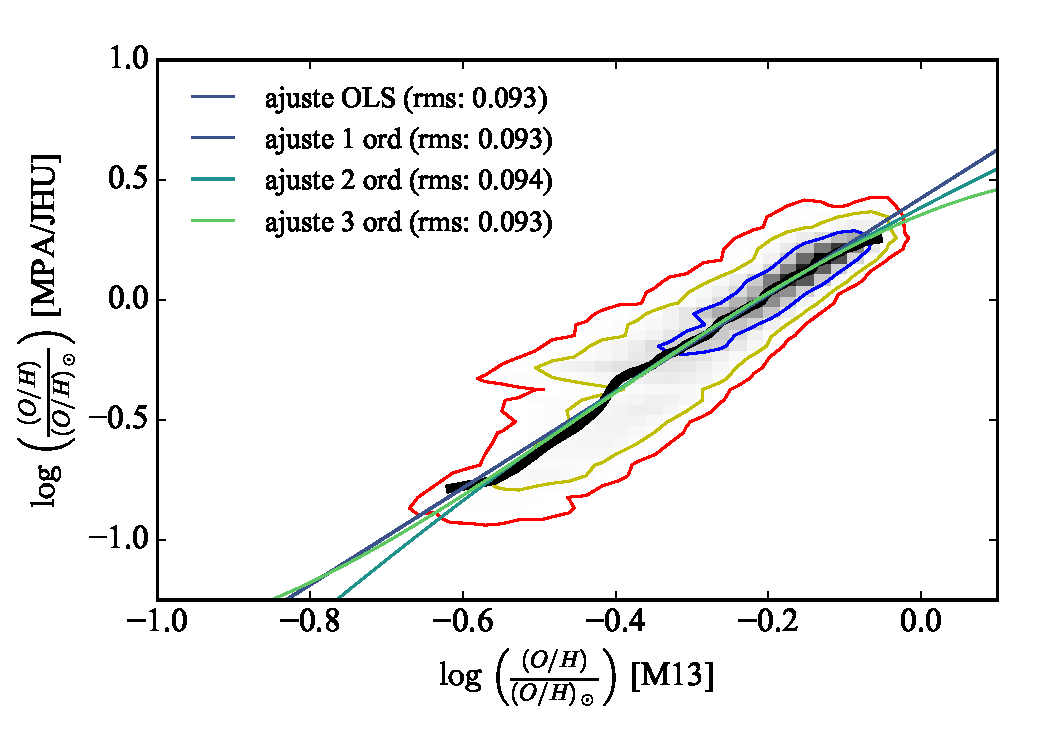
\includegraphics[width=0.9\textwidth]{figuras/logOH_ZnebMPA.pdf}
	\caption[Calibração das metalicidades.]
	{Calibração da metalicidade nebular (abundância relativa de oxigênio) do grupo MPA/JHU com a de
M13. A linha preta contínua representa a mediana da distribuição, as outras linhas, pelas cores
indicadas na legenda, são regressões polinomiais de $1^\underline{a}$, $2^\underline{a}$ e
$3^\underline{a}$ ordem e o {\em OLS bisector} da distribuição. Os contornos marcam $1\sigma$,
$2\sigma$ e $3\sigma$ respectivamente.}
	\label{fig:calibZ}
\end{figure}

\subsection{Analisando a conversão}
\label{sec:gasfrac:gas2dust:analisradperf}

Como não possuímos medidas diretas de gás de forma a validar a conversão vamos inverter a Eq.
\ref{eq:SFRKennicutt} para calcular $\SigmaGas$ a partir da KS. Através deste artifício podemos
verificar o comportamento assintótico de nossas variáveis calculadas ($\delta_{\mathrm{DGR}}$,
$\SigmaGas$, $f_{\mathrm{gas}}$). Vamos usar as seguintes equações para comparar:
\begin{eqnarray}
	\SigmaGas^{\mathrm{KS}} &=& \left(\frac{\SigmaSFR}{2.5 \times 10^{-4}}\right)^{\frac{1}{1.4}} \\
	\label{eq:SigmaGasKenn}
	\delta_{\mathrm{DGR}}^{\mathrm{KS}} &=& 0.2\ \left(\frac{\tauVS}{\SigmaGas^{\mathrm{KS}}}\right) \\
	\label{eq:DeltaDGRKenn}
	f_{\mathrm{gas}}^{\mathrm{KS}} &=& \frac{1}{1 +
	\left(\frac{\mu_\star}{\SigmaGas^{\mathrm{KS}}}\right)}.
	\label{eq:fGasKenn}
\end{eqnarray}
\noindent Juntamente produzimos a mesma versão destas variáveis, mas substituindo para os valores
nebulares quando possível ($\SigmaSFRN$ e $\tauVN$).

A Fig. \ref{fig:propsGasR} nos mostra os perfis radiais de $\delta_{\mathrm{DGR}}$, $\SigmaGas$ e
$f_{\mathrm{gas}}$. Apesar de que os perfis de $\delta_{\mathrm{DGR}}$ e $\SigmaGas$ parece
divergirem quanto ao comportamento ao longo do Raio, a fração de gás parece ser um resultado mais
robusto, graças a influência de densidade superficial de massa estelar ($\mu_\star$).
\begin{figure}
	\centering
	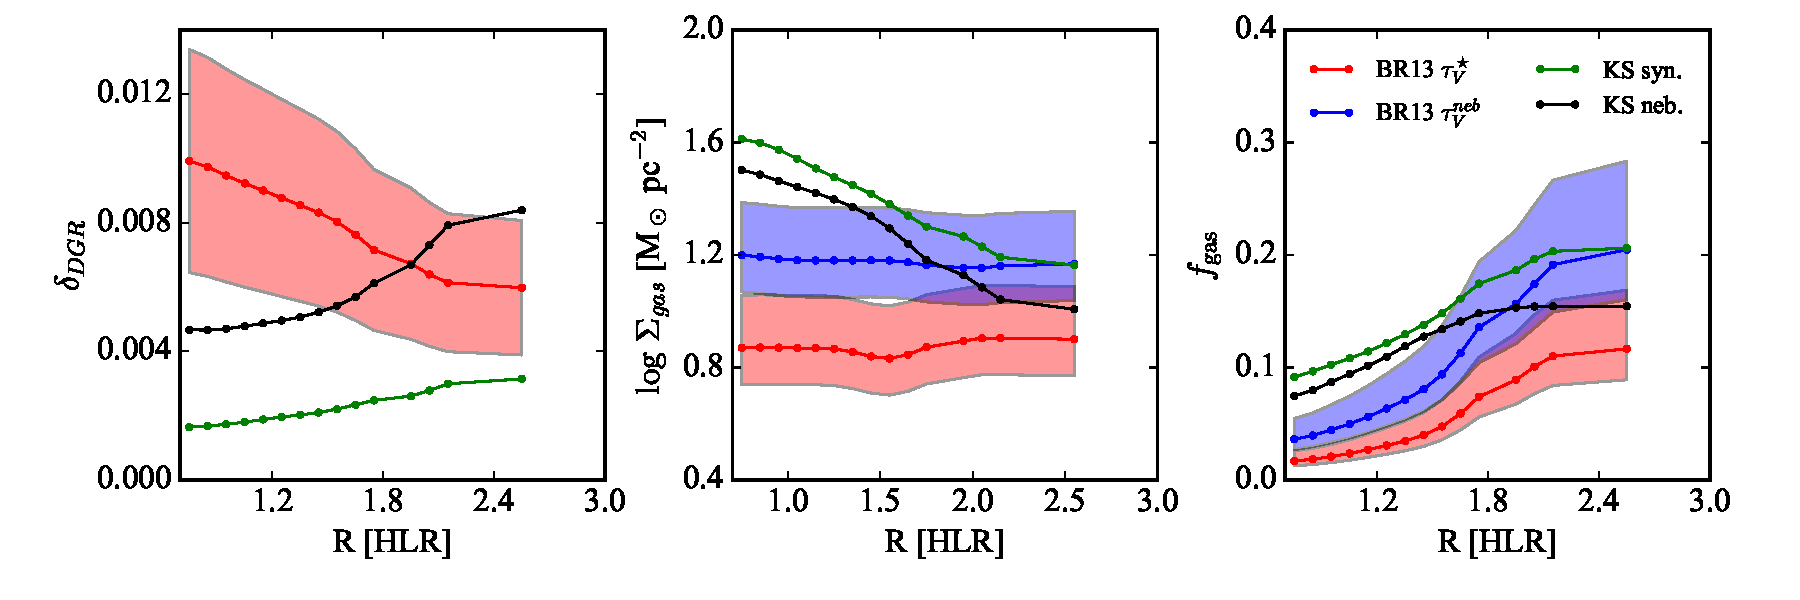
\includegraphics[width=0.99\textwidth]{figuras/gas_R.pdf}
	\caption[Perfis radiais de $\delta_{\mathrm{DGR}}$, $\SigmaGas$ e $f_{\mathrm{gas}}$.]
	{Perfis radiais para a razão poeira-gás ($\delta_{\mathrm{DGR}}$), densidade superficial de massa
de gás ($\SigmaGas$) e fração de gás ($f_{\mathrm{gas}}$). A área rachurada representa o intervalo
definido na Eq. \ref{eq:myDGR}. Em azul e vermelho temos a conversão de poeira em gás utilizando a
conversão pela Eq. \ref{eq:SigmaGasBR} com $\delta_{\mathrm{DGR}}$ definido na Eq. \ref{eq:myDGR},
utilizando $\tauVN$ e $\tauVS$ respectivamente. Em verde e preto temos as variáveis definidas no
início desta seção, invertendo a lei de KS, utilizando $\SigmaSFR$ e $\SigmaSFRN$.}
	\label{fig:propsGasR}
\end{figure}

\begin{figure}
	\centering
	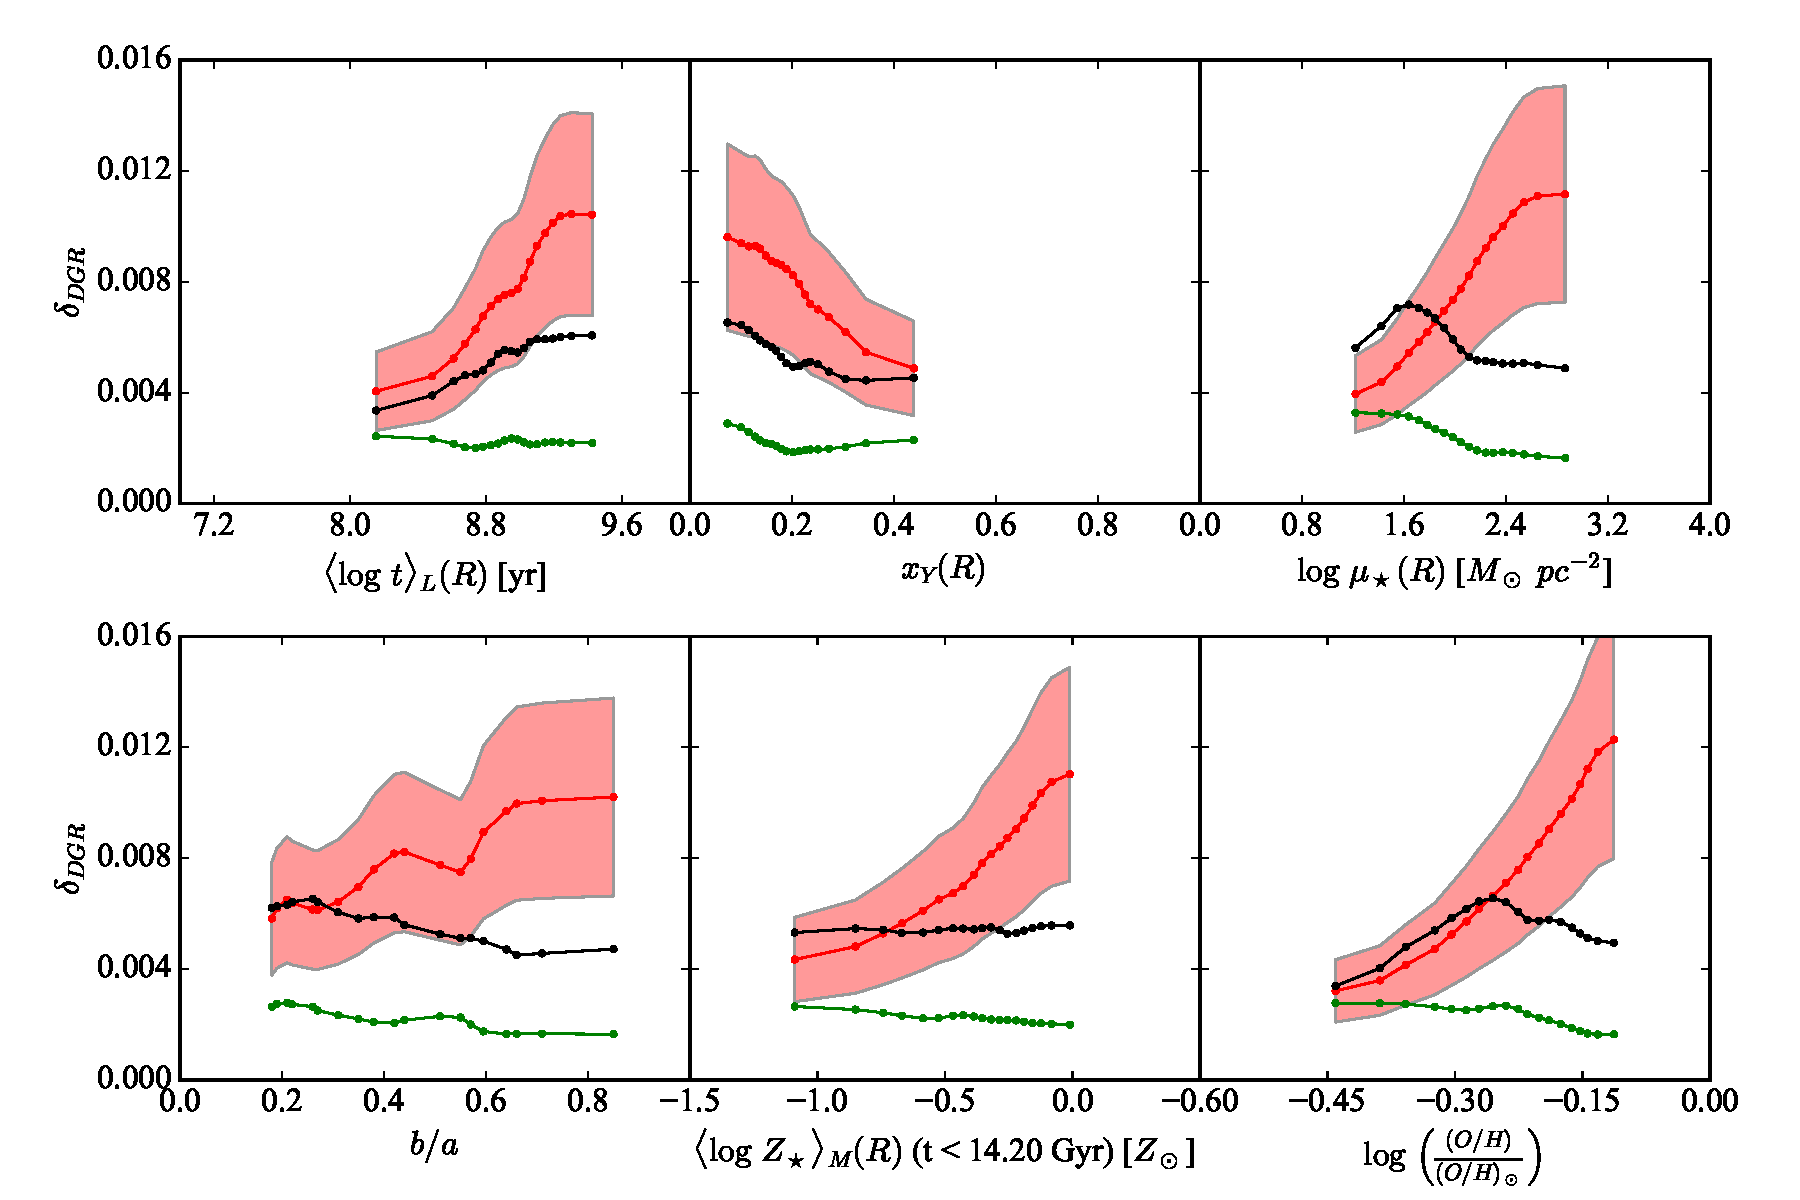
\includegraphics[width=0.99\textwidth]{figuras/props_DGR.pdf}
	\caption[Propriedades versos $\delta_{\mathrm{DGR}}$.]
	{}
	\label{fig:propsDGR}
\end{figure}
\begin{figure}
	\centering
	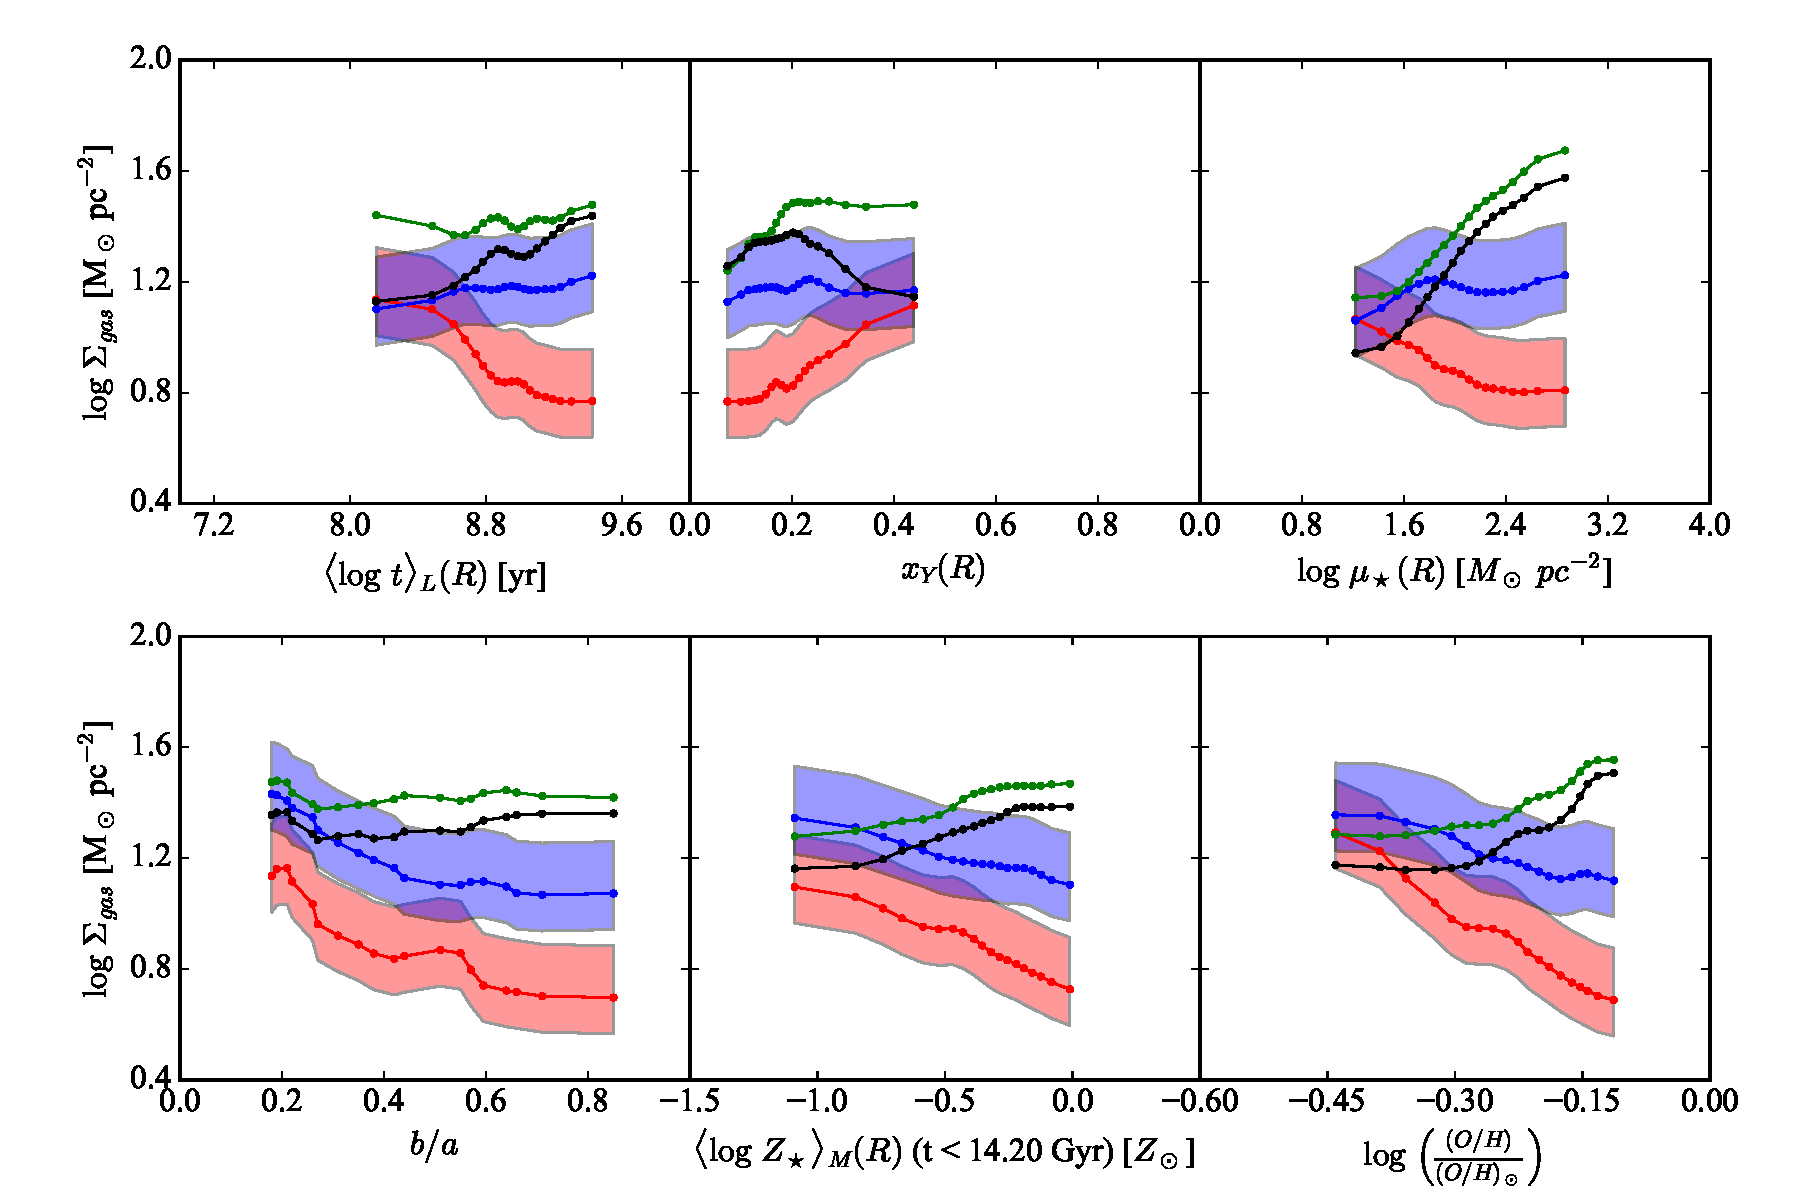
\includegraphics[width=0.99\textwidth]{figuras/props_SigmaGas.pdf}
	\caption[Propriedades versos $\SigmaGas$.]
	{}
	\label{fig:propsSigmaGas}
\end{figure}
\begin{figure}
	\centering
	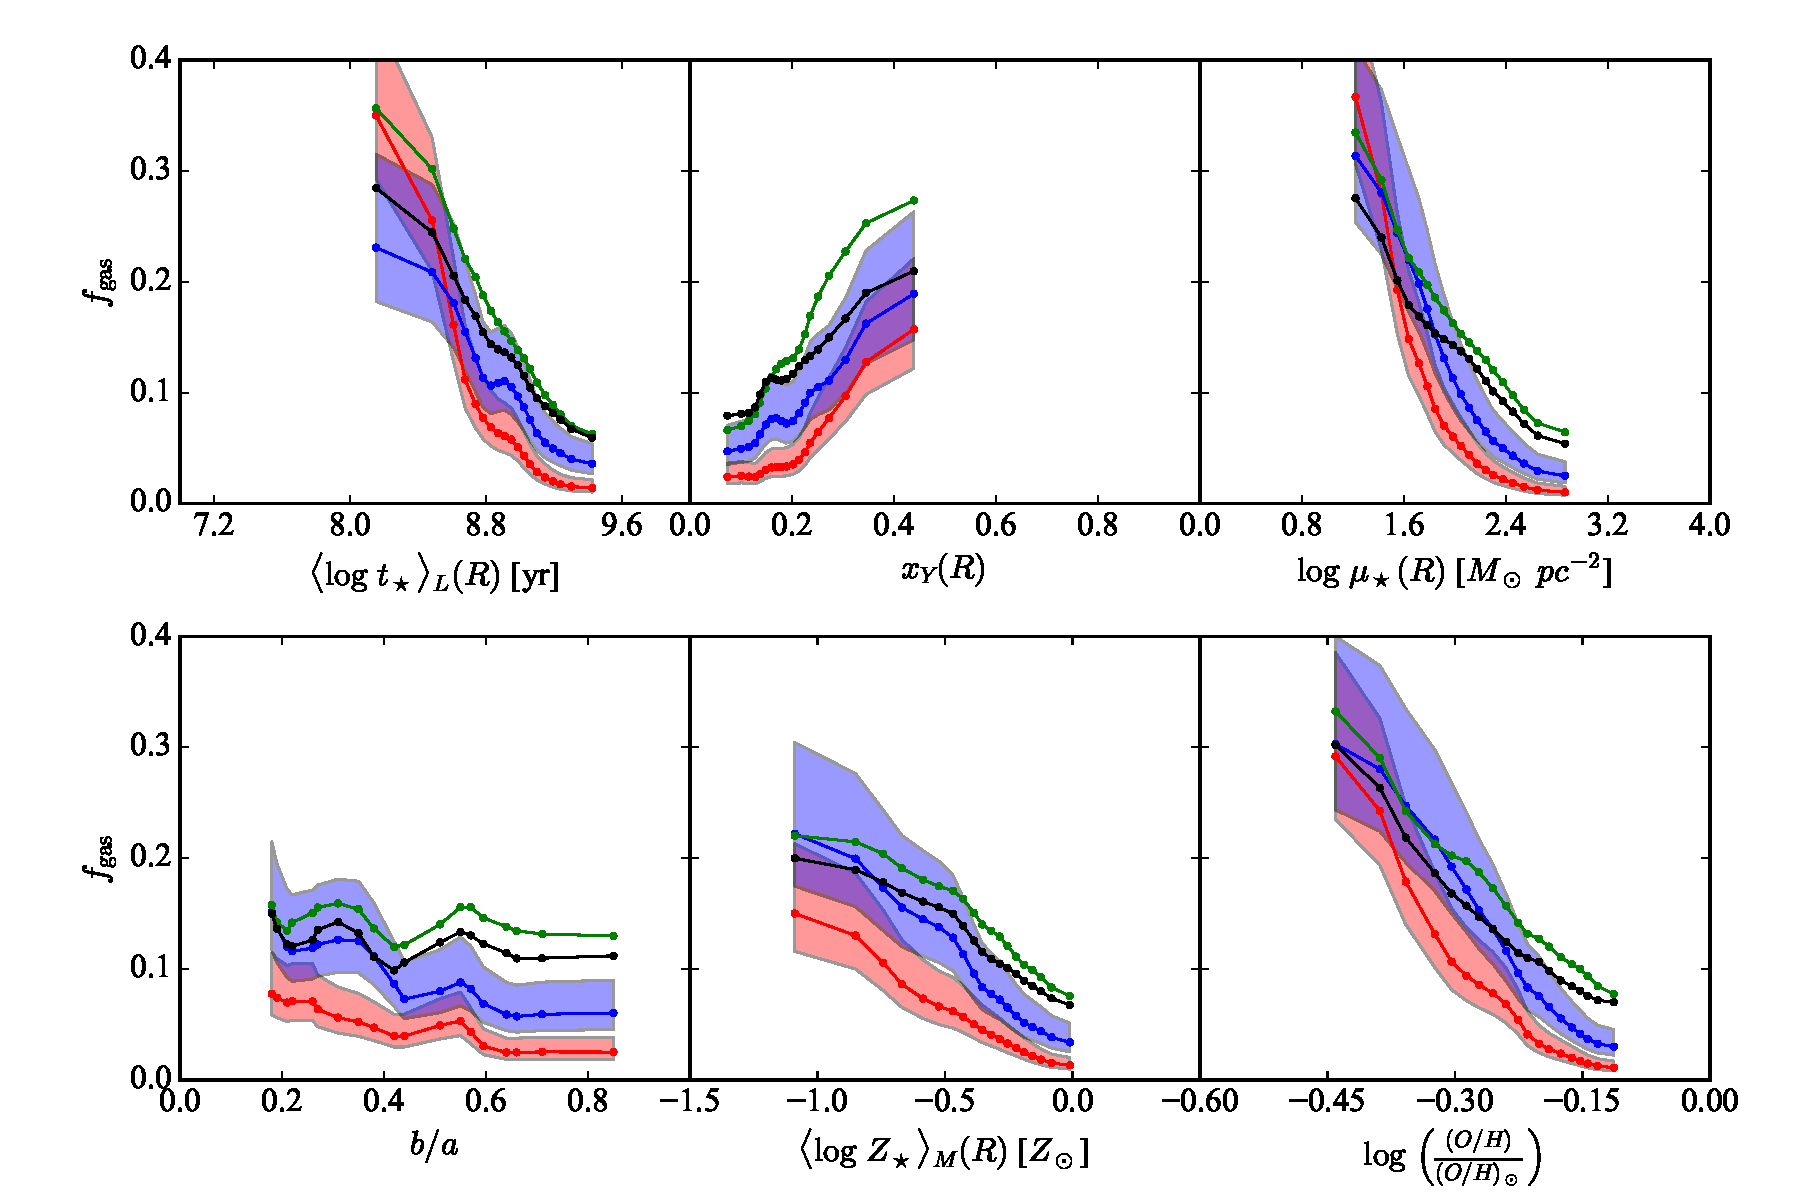
\includegraphics[width=0.99\textwidth]{figuras/props_fGas.pdf}
	\caption[Propriedades versos $f_{\mathrm{gas}}$.]
	{}
	\label{fig:propsfGas}
\end{figure}


\section{Eficiência e tempo de depleção do gás.}
\label{sec:gasfrac:SFE}

Um outro tipo de abordagem é trabalhar com a eficiência da transformação de gás em estrelas,
utilizando a relação:
\begin{equation}
	\mathrm{SFE} = \frac{\Sigma_{\mathrm{SFR}}}{\Sigma_{\mathrm{gas}}} = \frac{1}{t_{\mathrm{dep}}},
	\label{eq:SFE}
\end{equation}
\noindent onde SFE vem de {\em star-formation efficiency} e $t_{\mathrm{dep}}$, que é o inverso da
eficiência, é o tempo de depleção do gás, que nos dá uma ideia da escala de tempo em que a galáxia
consome todo o gás com a taxa em que está formando estrelas.

\ldots
%\chapter{Coeficiente de extinção como indicador de Gás}
%\label{sec:gas}
% Referências:
% - Brinchman
% - Guiderdoni & Rocca
% - procurar mais conversões dust to gas ou dust to stars
% - Referências para cada indicador
%\section{Indicadores de gás}
%\label{sec:synvsneb:proxies}
% Figuras:
% - ?? retiradas alguns papers para diferentes indicadores ??
%\section{Lei de Schimidt-Kennict}
%\label{sec:synvsneb:proxies}
% Figuras:
% - sample SK
% - our pseudo - SK
%\section{De poeira para gás}
%\label{sec:synvsneb:proxies}
% Figuras:
% - perfis radiais de SigmaGas e de fgas
% - real SK

% End of this chapter
